\label{sec:sokar-gui}

\par
Po uruchomieniu programu użytkownikowi ukazuje się główne okno, pokazane na rysuneku \ref{fig:sokar-gui-empty-window}, implementowane przez klasę \sokarclass{MainWindow}.
Okno zawiera 3 elementy: menu (obiekt klasy \qtclass{QMenuBar}), drzewo plików (obiekt klasy \sokarclass{FileTree}), obiekt zakładek z obrazami (obiekt klasy \sokarclass{DicomTabs}).

\begin{figure}[!htbp]
    \centering
    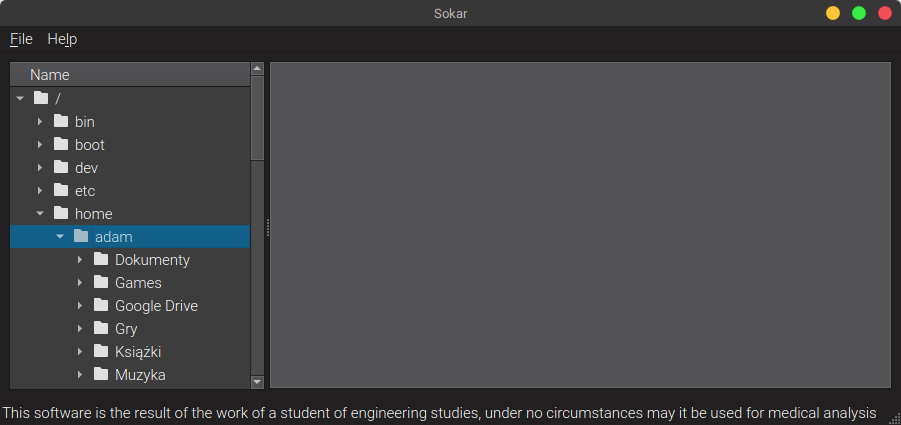
\includegraphics[width=0.7\textwidth]{img/sokar-gui-001.png}
    \caption{Okno przeglądarki tuż po uruchomieniu. Zdjęcie własne.}
    \label{fig:sokar-gui-empty-window}
\end{figure}

\par
Użytkownik może otworzyć plik \DICOM na trzy sposoby: z menu na górze, z drzewa ze strukturą plików lub poprzez przeciągnięcie \fromEng{drag and drop}.
W dwóch pierwszych przypadkach użytkownik może otworzyć tylko jeden plik, a w trzecim jest możliwość wczytania wielu plików.

\par
Po wczytaniu pliki są wyświetlane w zakładach.
Kontener z zakładkami jest implementowany przez klasę \sokarclass{DicomTabs}.
Przykład programu z wczytanymi kilkoma plikami, w tym jednym z animacją znajduje się na rysunku \ref{fig:sokar-gui-with-files}

\begin{figure}[!htbp]
    \centering
    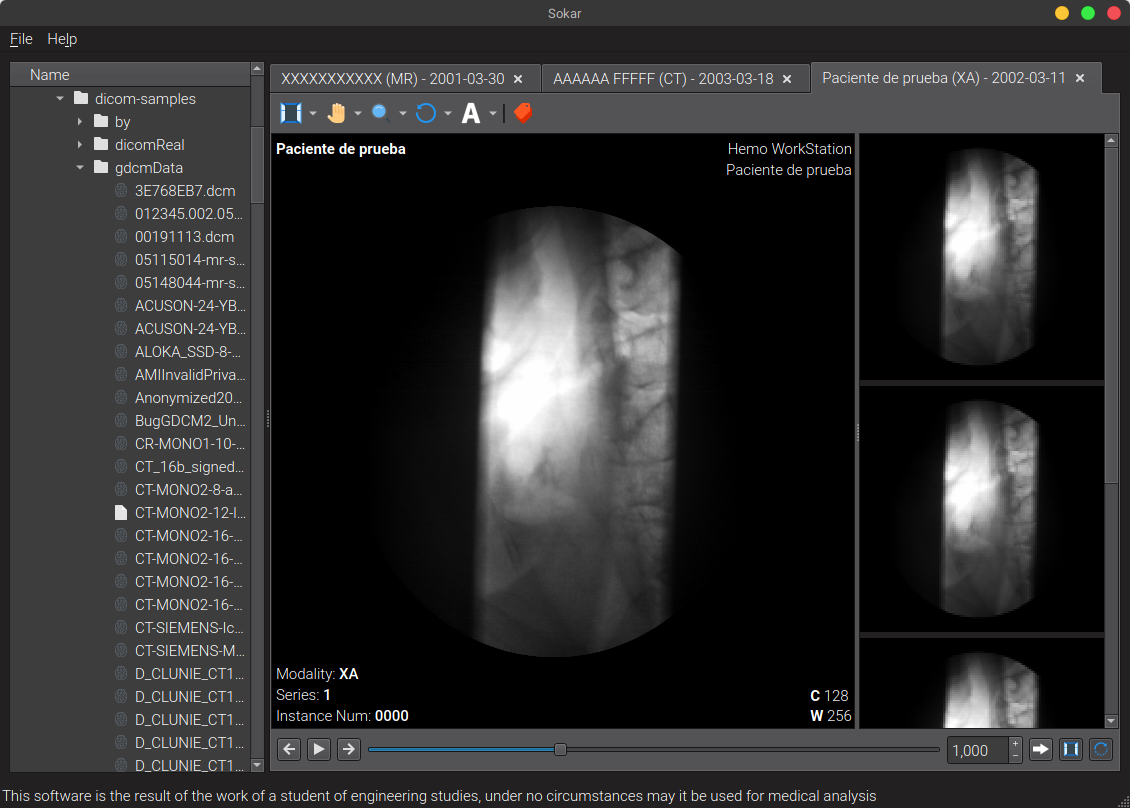
\includegraphics[width=\textwidth]{img/sokar-gui-002.png}
    \caption{Okno przeglądarki z wczytanymi kilkoma obrazami. Zdjęcie własne.}
    \label{fig:sokar-gui-with-files}
\end{figure}

\par
Obiekt wewnątrz zakładek odpowiada za wyświetlanie wszystkich elementów umożliwiających interakcje użytkownika z obrazem.
Jest on implementowany przez klasę \sokarclass{DicomView}.
Jeden taki obiekt może posiadać wiele obrazów wyświetlanych w formie animacji.
Obrazy są wyświetlane na scenie implementowanej przez \sokarclass{DicomScene}.
Pod sceną znajduje się pasek filmu z pomocą, którego użytkownik może zatrzymać lub wznowić animację.
Na prawo od sceny znajdują się ikony i z wszystkimi ramkami filmu.
Pasek filmu i ikony obrazów ukrywają się, gdy jest wczytany tylko jeden obraz.
\par
Scena to obiekt wyświetlający i generujący obraz na ekranie.
Dodatkowo na scenie znajduję się pięć zestawów informacji z pliku \DICOM:
\begin{itemize}
    \item dane pacjenta w lewym górnym rogu
    \item dane szpitala lub jednostki w której obraz został wykonany w prawym górnym rogu
    \item dane akwizycji obrazów w lewym dolnym rogu, mogących sie różnić dla każdej modalności
    \item podziałka informująca o rzeczywistym rozmiarze obiektu znajdującego się na obrazie znajdująca się w dolnej i prawej części obrazu
    \item cztery litery z sześciu (H, F, A, P, R, L) informujących o ułożeniu obrazu względem pacjenta
\end{itemize}
Przykładowa scena z obrazem monochromatycznym znajduje sie na rysunku \ref{fig:sokar-gui-scene}.

\begin{figure}[!htbp]
    \centering
    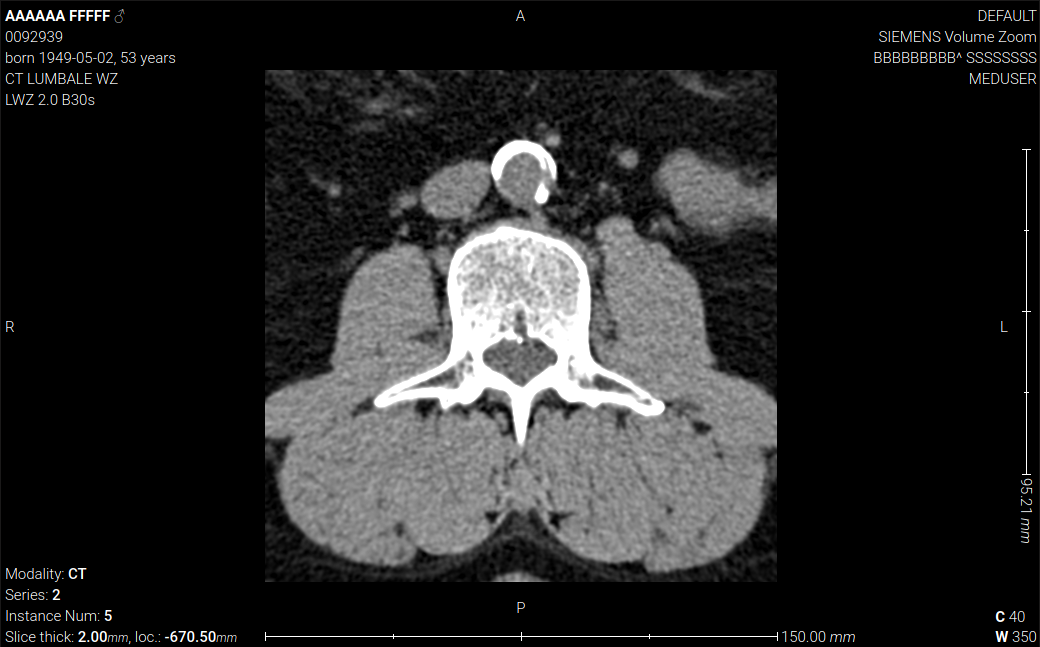
\includegraphics[width=\textwidth]{img/sokar-gui-003.png}
    \caption{Przykładowa scena z obrazem monochromatycznym. Zdjęcie własne.}
    \label{fig:sokar-gui-scene}
\end{figure}

\par
Możliwość wyświetlania animacji pojawia się wtedy, gdy w jednej zakładce będzie znajdowała się więcej niż jedna ramka obrazu.
Można to osiągnąć wczytując wiele obrazów z tej samej serii lub wczytać obraz posiadający wiele ramek.
Wówczas pod sceną pojawia się pasek, umożliwiający sterowanie animacją, a po prawej stronie obiekt z ikonami poszczególnych ramek obrazu.
Dokładny opis przycisków i ich funkcji znajduje się w sekcji.
\par
Pełna struktura menu programu znajdującego się na górze jest opisana w sekcji \ref{sec:sokar-window-menu}.